% Based on the "sig-alternate.tex" V2.1 April 2013
% This file should be compiled with V2.5 of "sig-alternate.cls" May 2012
% For tracking purposes - this is V2.0 - May 2012

\documentclass{sig-alternate-05-2015}


\begin{document}

% Copyright
\setcopyright{acmcopyright}
%\setcopyright{acmlicensed}
%\setcopyright{rightsretained}
%\setcopyright{usgov}
%\setcopyright{usgovmixed}
%\setcopyright{cagov}
%\setcopyright{cagovmixed}


% DOI
%\doi{10.475/123_4}

% ISBN
%\isbn{123-4567-24-567/08/06}

%Conference
\conferenceinfo{WWW}{2017 Perth, Western Australia, Australia}

\acmPrice{\$15.00}

%
% --- Author Metadata here ---
\conferenceinfo{WWW}{2017 Perth, Western Australia, Australia}
%\CopyrightYear{2007} % Allows default copyright year (20XX) to be over-ridden - IF NEED BE.
%\crdata{0-12345-67-8/90/01}  % Allows default copyright data (0-89791-88-6/97/05) to be over-ridden - IF NEED BE.
% --- End of Author Metadata ---

\title{Automatic Supplemental Content Suggestions in Hypertext Editors using a Semantic Knowledge Graph
\titlenote{A full version of this paper is available at
https://w3id.org/people/prototypo/papers/WWW2017a}}
%
\numberofauthors{3} % REQUIRED for 3-column layout.
%
\author{
% 1st. author
\alignauthor
David Hyland-Wood\\
       \affaddr{Ephox Corporation}\\
       \affaddr{225 Montague Road, Level 4}\\
       \affaddr{West End, Queensland, Australia}\\
       \email{david.wood@ephox.com}
% 2nd. author
\alignauthor
Anna Harrison\\
       \affaddr{Ephox Corporation}\\
       \affaddr{225 Montague Road, Level 4}\\
       \affaddr{West End, Queensland, Australia}\\
       \email{anna.harrison@ephox.com}
% 3rd. author
\alignauthor
Ben Kolera\\
       \affaddr{Ephox Corporation}\\
       \affaddr{225 Montague Road, Level 4}\\
       \affaddr{West End, Queensland, Australia}\\
       \email{ben.kolera@ephox.com}
}

\maketitle
\begin{abstract}
Many types of writing, such as blog posts and business documents, could benefit from supplemental explanatory material to provide context, background, and additional information for exploration. The World Wide Web provides huge quantities of such supplementary material, but it is not generally suitable for inclusion in new writing due to issues of licensing, copyright, formatting, or syntax. Exceptions include clearly identifiable content meant to be embedded in hypertext documents, such as YouTube videos, and Twitter feeds. We demonstrate how the textual content in a general purpose hypertext editor may be used to automatically identify relevant supplementary material via artificial intelligence (AI) processes, and that material may be presented to a document author for possible inclusion in whole or in part. User interface elements are provided to allow an author to refine content suggestions with a minimum of input.
\end{abstract}


%
% The code below should be generated by the tool at
% http://dl.acm.org/ccs.cfm
% Please copy and paste the code instead of the example below. 
%
\begin{CCSXML}
<ccs2012>
<concept>
<concept_id>10010147.10010178.10010187.10010188</concept_id>
<concept_desc>Computing methodologies~Semantic networks</concept_desc>
<concept_significance>500</concept_significance>
</concept>
<concept>
<concept_id>10003120.10003123.10011759</concept_id>
<concept_desc>Human-centered computing~Empirical studies in interaction design</concept_desc>
<concept_significance>500</concept_significance>
</concept>
<concept>
<concept_id>10003456.10003457.10003567.10010990</concept_id>
<concept_desc>Social and professional topics~Socio-technical systems</concept_desc>
<concept_significance>300</concept_significance>
</concept>
<concept>
<concept_id>10010405.10010497.10010510.10010920</concept_id>
<concept_desc>Applied computing~Hypertext / hypermedia creation</concept_desc>
<concept_significance>300</concept_significance>
</concept>
</ccs2012>
\end{CCSXML}

\ccsdesc[500]{Computing methodologies~Semantic networks}
\ccsdesc[500]{Human-centered computing~Empirical studies in interaction design}
\ccsdesc[300]{Social and professional topics~Socio-technical systems}
\ccsdesc[300]{Applied computing~Hypertext / hypermedia creation}


%
% End generated code
%

%
%  Use this command to print the description
%
\printccsdesc

% We no longer use \terms command
%\terms{Theory}

\keywords{ACM proceedings; RDF; knowledge graph; Linked Data; IBM Watson}

\section{Introduction}
Many types of writing, such as blog posts and business documents, could benefit from supplemental explanatory material to provide context, background, and additional information for exploration. The World Wide Web provides huge quantities of such supplementary material, but it is not generally suitable for inclusion in new writing due to issues of licensing, copyright, formatting, or syntax. Exceptions include clearly identifiable content meant to be embedded in hypertext documents, such as YouTube videos, and Twitter feeds.

We wanted to determine whether the textual content in a general purpose hypertext editor may be used to automatically identify relevant supplementary material via artificial intelligence (AI) processes, and whether that material may be presented to a document author for possible inclusion in a document in a useful manner.

The techniques necessary for such an exploration are now generally available. Linguistic parsing of text content may be conducted relatively easily using generally available tools, at least in many European languages including English. Concept identification from the results of linguistic parsing has been similarly successful.

Concepts may be matched to relevant additional information by querying a graph of information in the Resource Description Framework (RDF) data model\cite{cyganiak2014rdf}. Such information form ``knowledge graphs" of related information.

The first general purpose knowledge graph of scale was Freebase\cite{bollacker2008freebase}, which became the basis for the Google Knowledge Graph\cite{singhalintroducing}. Web search engines such as Google, Bing, and Yandex now use knowledge graphs to provide summaries of relevant information related to search terms. It is exactly this functionality that we wanted to add to our general purpose hypertext editors.

During the writing of this paper, Google announced a feature similar to the one described in this paper for their vertically-integrated Google Docs product\cite{googledocsexplore}. The Google Docs ``Explore'' button opens a sidebar that exposes a search option, and presents concepts, images, and related information. Images may be dragged into a document; other presented content opens Web pages for further reading.

\section{Architecture}

\begin{figure*}
\centering
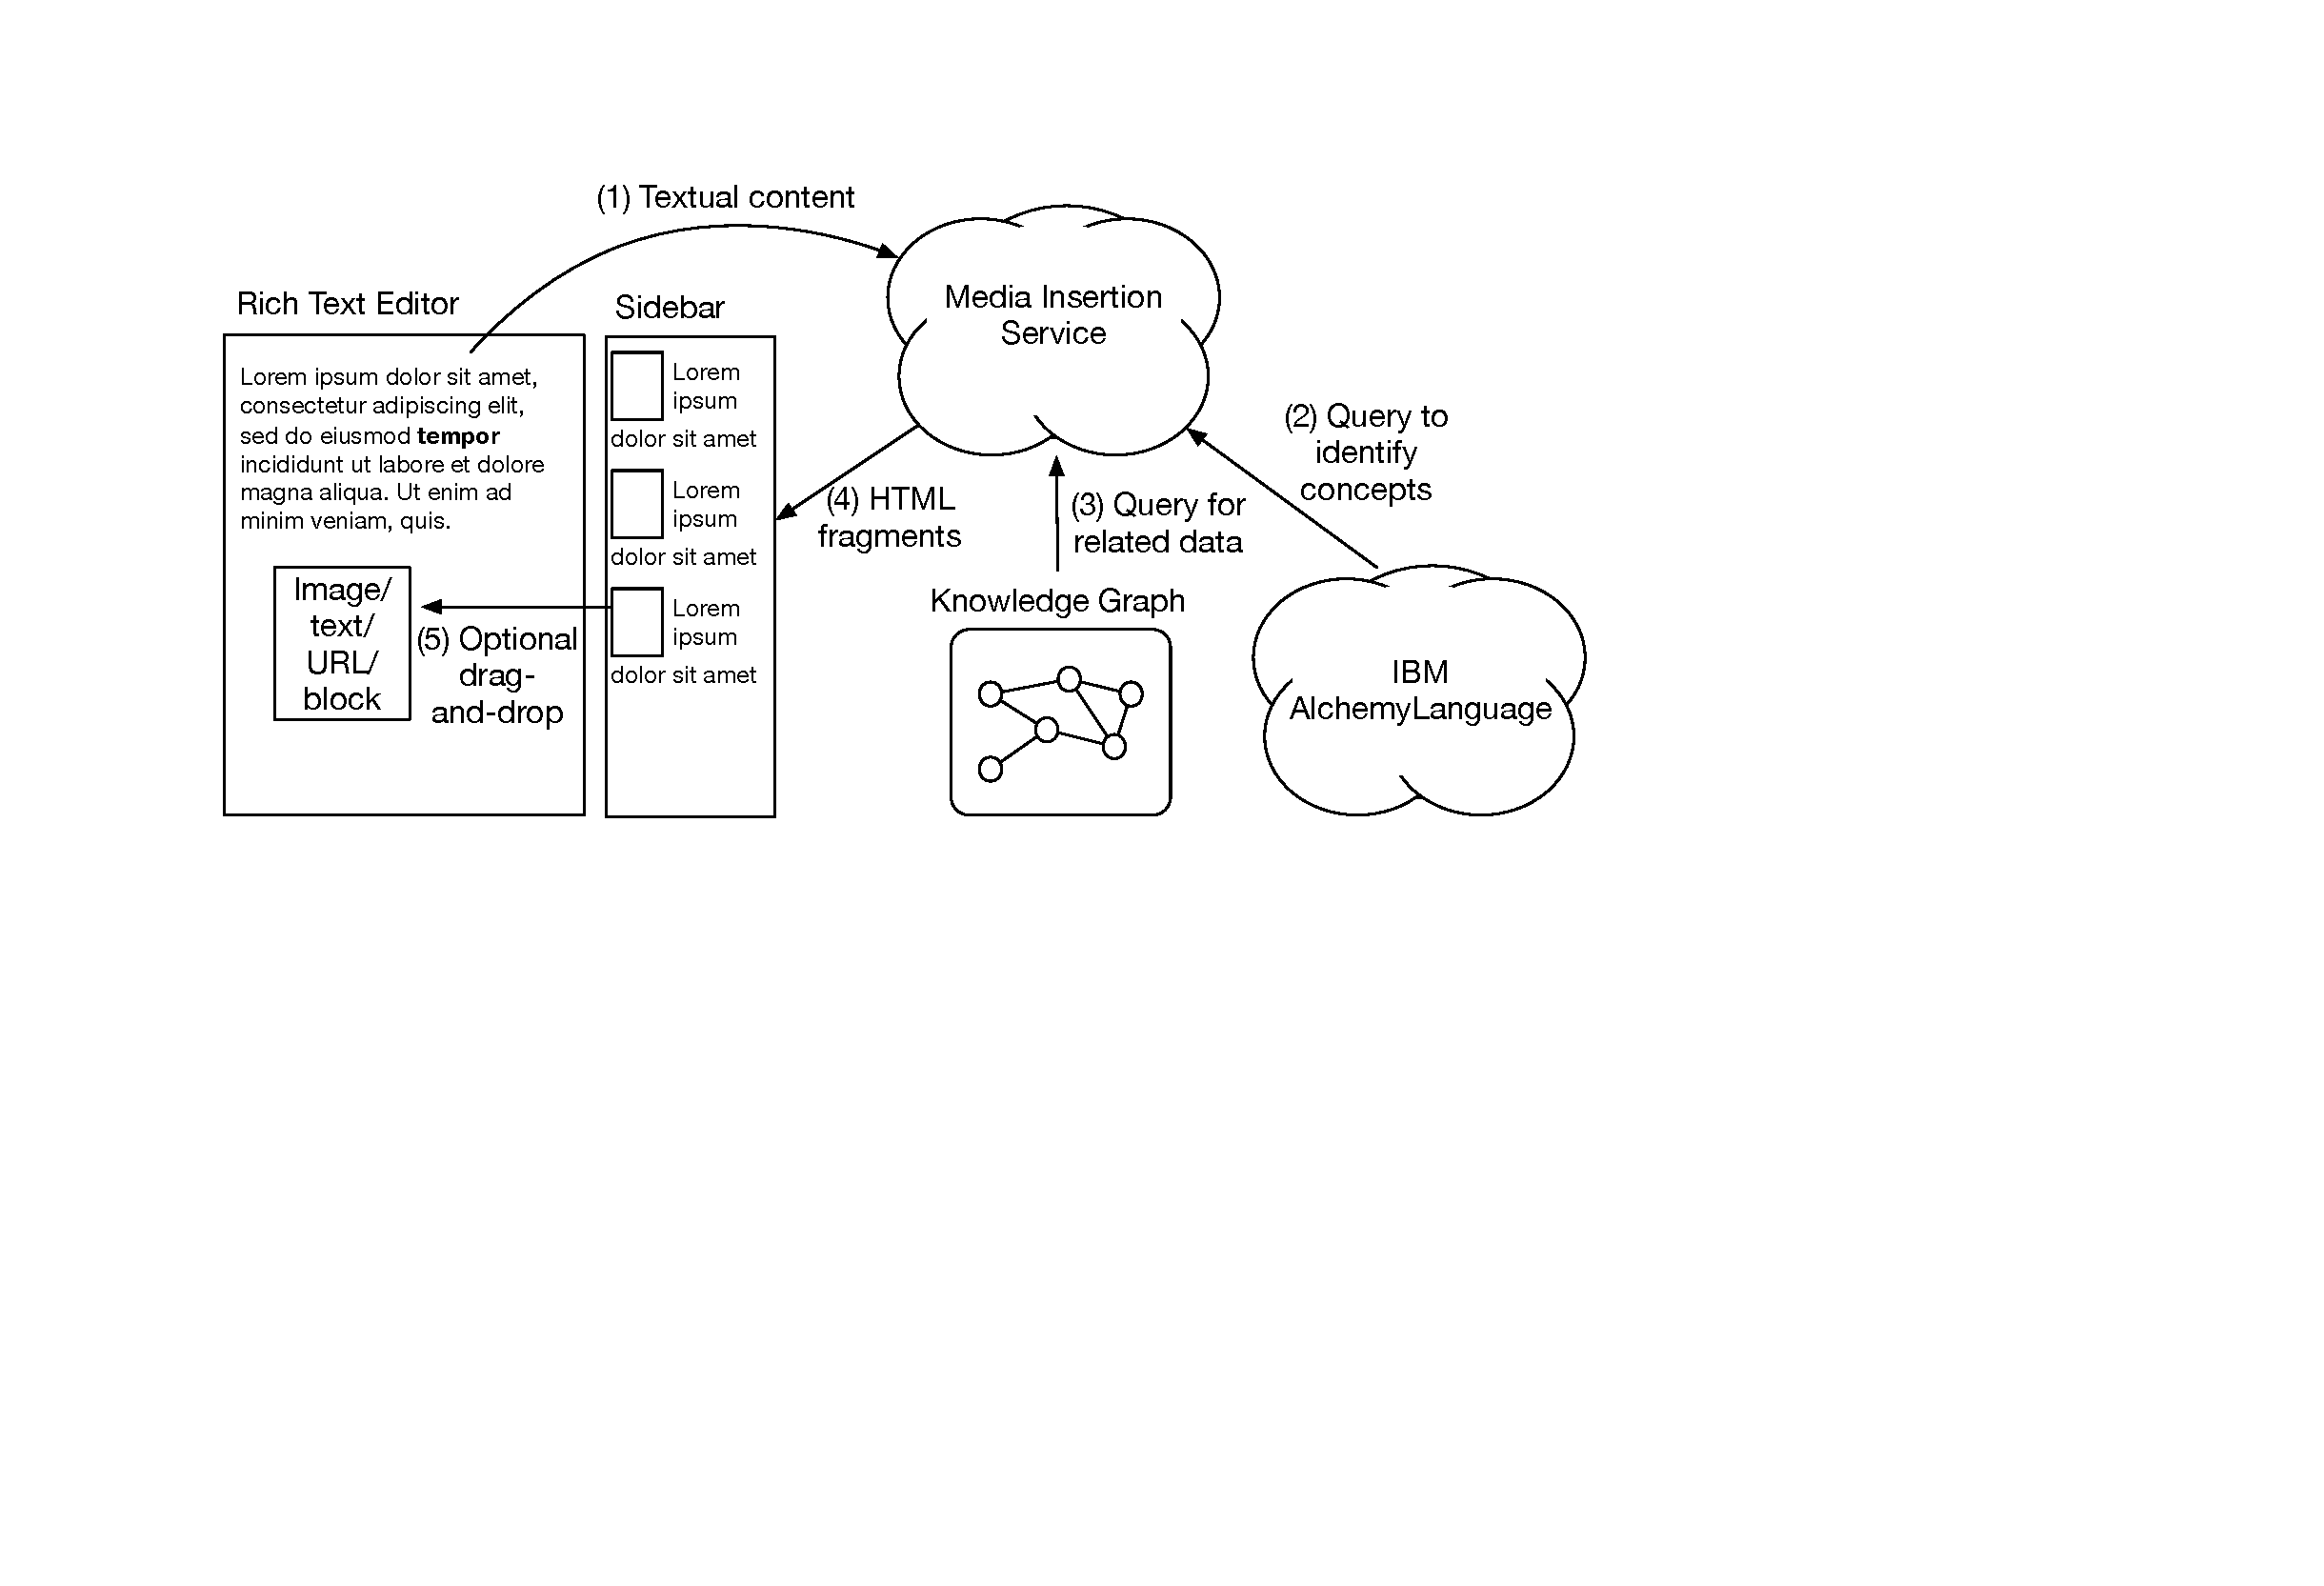
\includegraphics[scale=0.6]{images/KGarchitecture}
\caption{Data flow from editor to sidebar via enhancement services.}
\label{fig:architecture}
\end{figure*}

We wrapped one of our JavaScript hypertext editors, Text\allowbreak{}box.io, to include a sidebar for the presentation of supplemental material. The sidebar is a simple HTML component that accepts HTML fragments for display and possible drag-and-drop of components into the editor's content pane. JavaScript is used to query on online service to search for relevant information based upon the current contents of the editor.

Textual content is written into the editor by a document author. That content is uploaded to an Ephox cloud service for analysis (Figure \ref{fig:architecture}). The Ephox service sends the content to another service to parse the content, and extract concepts. We used IBM's online AlchemyLanguage service\footnote{\texttt{http://www.alchemyapi.com/products/alchemylanguage/}} for linguistic parsing and concept identification, although any number of similar services could have been used for those purposes. AlchemyLanguage is based upon IBM's Watson question-answering AI system\cite{ferrucci2010building}.

One advantage of the AlchemyLanguage API is that its concept tagging service\footnote{\texttt{http://www.alchemyapi.com/products/alchemylanguage/\allowbreak{}concept-tagging}} returns DBpedia\cite{auer2007dbpedia}, Yago\cite{suchanek2008yago} and Freebase URIs for each identified concept. We used DBpedia URIs as indexes into an RDF knowledge graph.

To implement our knowledge graph service, we used an Apache Tomcat\footnote{\texttt{https://tomcat.apache.org/}} Web application server with a RDF4J\footnote{\texttt{http://rdf4j.org/}} version 2.0 RDF database engine. Relevant portions of DBpedia were sharded into six RDF4J databases to speed both data indexing and assist query performance. DBpedia topical concepts, SKOS\cite{miles2009skos} categories, labels, image URLs, short abstracts, categories and their labels, transitive instance types, mapping-based objects and literals, and person data were used for our initial experiments. We limited our DBpedia extracts to the English language due to the language limitations of the AlchemyLanguage concept tagging service.

Two SPARQL 1.1\cite{harris2013sparql} queries against the knowledge graph were used to construct supplemental material representations:

\begin{itemize}
\item The first SPARQL query is used to identify the type of a concept (i.e. each concept will be either a person, place, organization, movie, species, product, or a general concept).
\item The second SPARQL query is used to identify available data about a specific concept, as anticipated by its type.
\end{itemize}

Thus, a concept of type ``person" might have a birth date and a birth place. A place might have area and a population estimate, etc. Most data elements for any given type are considered to be optional.

The results of the second query are used to fill a type-specific HTML template. An HTML fragment is produced for each concept, and any empty divs are removed. The completed fragment is returned to the editor's sidebar for display.

SPARQL 1.1 SERVICE clauses were used to execute federated queries\cite{prud2013sparql} across the various databases making up the knowledge graph.

We chose to construct our own knowledge graph instead of using one provided by the AlchemyLanguage service. We wish to eventually refine and contextualize the contents of the knowledge graph over time to provide industry- or even customer-specific data. We also wanted to be able to swap linguistic parsing and concept tagging services if desired at a later time.

A sidebar was added to our editors. Relevant components are illustrated in in Figure \ref{fig:sidebar-terms}. The show/hide button (2) opens and closes the sidebar panel, shrinking the main editor window content area (1) as it does so. The text typed into the main content area (1) is sent to the server for processing, and the top five concepts returned displayed as keywords (3) in the sidebar area. Individual concepts related to the search terms (3) are displayed as concept widgets (4). Each concept widget has a title and a combination of media and text items. Actions such as view and insert are displayed as buttons at the bottom of each concept widget (6). The concept widgets (4) and media items (5) are able to be drag and dropped into the main content area (1).

\begin{figure*}
\centering
\includegraphics[scale=0.85]{images/sidebar-terms}
\caption{Editor and sidebar user interface elements.}
\label{fig:sidebar-terms}
\end{figure*}

\section{Usage}
\label{sec:usage}

\begin{figure*}
\centering
\includegraphics[scale=0.35]{images/DndOfSidebarContent}
\caption{One possible interaction mode; drag-and-drop of suggested content. Content may be reformatted to match editor settings.}
\label{fig:DndOfSidebarContent}
\end{figure*}

We developed several interaction modalities to facilitate the adding of supplemental material to textual content in the editor. Specifically, we implemented five different types of interactions:

\begin{enumerate}
\item \textit{Link insertion}. Inserts a link to the knowledge graph concept.
\item \textit{Panel insertion}. Inserts the linked knowledge graph concept widget as an in-line formatted blockquote.
\item \textit{Media insertion}. Inserts the media (image or video) from the knowledge graph concept widget into the document.
\item \textit{Concept filtering}. Removes concept search terms from the search query.
\item \textit{Link viewing}. Opens the link to the knowledge graph concept in a separate browser window.
\end{enumerate}

Each interaction type is described below.

\subsection{Link insertion}

The first interaction type we implemented was the ability to simply add a link to the knowledge graph concept from the sidebar directly into the document. This functionality was delivered through an \texttt{Insert link} button on each concept widget. Pressing the \texttt{Insert link} button would insert a link at the current cursor position, or, if a selection was made in the editor the link would be applied to the selected text.

\subsection{Panel Insertion}

The panel insertion interaction was implemented using two interaction styles. Firstly, like link insertion, a panel could be inserted into the document by clicking the \texttt{Insert panel} button on each concept widget. In addition, a drag-and-drop interaction was implemented on the panel, allowing the concept widget to be dragged directly into the document. In both cases, the resulting concept was displayed as a formatted, in-line blockquote.

\subsection{Media insertion}

The media insertion interaction was provided as a drag-and-drop interaction only, with no corresponding button on the concept widget. In this case, selecting a specific image (or video) from the sidebar and dragging it into the document embedded the media item only in-line in the document, the formatted blockquote was not included.

\subsection{Concept filtering}

Concept filtering was implemented using two different interaction elements. The first element listed the top five concepts identified by the AI service as keywords at the top of the sidebar area. Each concept could be removed from consideration by deselecting its visual tag. Removal of a concept from the user interface removes it from the knowledge graph search. In the example below, closing ``The Bronx" concept keyword results in that term being removed from the search, and all concept widgets related to that term being removed from the sidebar.

\begin{figure}
\includegraphics[scale=0.35]{images/concept-filtering}
\caption{Concept filtering interaction sequence.}
\label{fig:concept-filtering}
\end{figure}

\textbf{TODO:} Does the following paragraph belong? Should it be rewritten?

A secondary concept filter was implemented on each concept widget. This filter closed individual concept widgets, but did not remove the concept from the set of terms being searched. In the third panel above, closing the ``Long Island" panel removes it from the sidebar, but does not remove ``Long Island" from the list of terms being searched, i.e. other information related to Long Island could still appear in the sidebar.

\subsection{Link viewing}

The final interaction modality implemented allowed the viewing of the original knowledge graph concept in a new browser window. This was implemented as a \texttt{View link} button on each concept widget, and also as a hyperlink from the concept title. In both cases, clicking the button or the link opened the Wikipedia page related to the knowledge graph concept in a new browser tab.


\section{Evaluation}

We ran an unmoderated observational research study in order to test the usage model described in the previous section. Participants were given a writing task and asked to enrich their writing using the Cognitive Assistant. The task description given to users was:

\begin{quote}
Your Task: Imagine you are writing a blog post to tell your friends about a holiday you recently took (or would like to take) to New York City. Write your story in the editor window below.

Using the Cognitive Assistant, enhance your story with:

\begin{enumerate}
\item Information about the city itself
\item Information about any attractions, landmarks, shows, movies or restaurants that you visited (or would like to visit).
\item Information about famous sports teams based in New York City
\end{enumerate}

Please include at least one quote and one video.
\end{quote}

The test task intentionally did not prompt the participants on how to achieve the task as we were interested in exploring the natural way in which participants would interact with the sidebar element. Participants were instructed to use a ``talk aloud" protocol while completing the task and their interactions recorded using the online testing service Validately.com.

The test was deployed to 20 participants aged over 18 years old and having some university education. Of the 20 participants, 11 were female and 9 were male. Of the 20 deployed tests, 13 were completed either in whole or in part.

\section{Results}

\begin{table*}
\centering
\caption{Results from user tests}
\label{table:results}
\begin{tabular}{|l|c|c|c|} \hline
Results for completed tests, n=13&DISCOVERABLE&INTUITIVE&USEFUL\\ \hline
All interactions (1, 2, 3, 4 5), n=35 & 54\% & 39\% & 32\% \\ \hline
Any insert interaction (1 or  2 or  3), n=13 & 100\% & 92\% & 85\% \\ \hline
Concept filtering interaction (4), n=11 & 85\% & 31\% & 8\% \\ \hline
Link viewing interaction (5), n=2 & 16\% & 16\% & 16\% \\ \hline
\end{tabular}
\end{table*}

The videos results were coded against the five-part usage model described in section~\ref{sec:usage}, namely: (1) link insertion; (2) panel insertion; (3) media insertion; (4) concept filtering and (5) link viewing. For each of these categories, two of the authors independently evaluated whether the participant:

\begin{enumerate}
\item Found the interaction modality (DISCOVERABLE)
\item Was able to interact in an intuitive way (INTUITIVE)
\item Perceived the interaction as having value (USEFUL) 
\end{enumerate}

The results were triangulated and discrepancies resolved by reviewing the video footage. Results are shown in Table~\ref{table:results}.

\textbf{TODO:} Add PURL link to summary video.

\subsection{All interactions}

Most participants intuited what the sidebar represented. Some representative comments included:

\begin{quote}
Looking at this cognitive assistant, that is interesting. The internet tells me a lot, about what New York is about, and I can insert it right here. It gives me a lot of extra information that I need, and it makes writing very simple because it's integrated.
\end{quote}

\begin{quote}
...this is a great concept! I love the idea of a search engine running in the background, finding information to strengthen my writing. 
\end{quote}

\begin{quote}
This readily helps me to create a blog as it makes it very easy and quick to write... and it guides me with information that inspires me to write more, so I don't have writers block. It's very intuitive, and helps me to write a story with an abundance of information for the viewers of my blog.
\end{quote}

\begin{quote}
[opens cognitive assistant] Oh, how interesting! So it looks like, maybe it searched the text [in the document] and used a search engine to look up the information from my text. That's very interesting.
\end{quote}

12 of the 13 participants who completed the task were able to interact with the sidebar to varying degrees of success: the majority of interaction modalities were engaged with (54\%), over a third (39\%) of the interactions appeared intuitive and around a third (32\%) appeared useful.

A few participants commented on the sidebar being a source of inspiration for ideas that they had not thought of themselves.

\begin{quote}
The New York Giants... actually I don't follow sports so I will use the cognitive enhancer [to get some info on this topic].
\end{quote}

\begin{quote}
[on opening cognitive assistant] Oh that's cool. It shows me facts about the Statue of Liberty... I like this system, how you can get facts on what you are typing about.
\end{quote}

\subsection{Any insert interactions}

The three interaction modalities (link, panel and media insertion) were implemented as alternate modes of interaction. Looking at the results, all of the participants (100\%) figured out some way to interact with the sidebar in an intuitive way (92\%), and most found these interactions useful (85\%). 

Link insertion was the least engaged with mode of interaction: only 3 of the 13 participants directly inserted a link using the \texttt{Insert link} button on the concept widget. 9 out of the 13 participants intuitively inserted a panel from the sidebar into their document (using either drag and drop or pressing the \texttt{Insert panel} link). Media insertion was the most intuitive interaction mode, with 10 out of 13 participants dragging media from the sidebar into the document. This result suggests that incorporating images and videos into the concept widgets in the sidebar will promote interaction (as opposed to text-only concept widgets).

For some, while analysis of their interactions revealed that they interacted with the sidebar as expected, their words provided a different narrative:

\begin{quote}
[uses the cognitive assistant to successfully insert a video and a concept panel] I'm going to say that because it was a prototype, I was unable to use the cognitive assistant
\end{quote}

The above result is not uncommon in this type of testing, and underscores the benefits of observational research over survey-style methods: i.e. the truth lies in what participants do, not what they say that they do.

\subsection{Concept filtering}

The concept filtering interaction modality was discovered by 85\% of participants, however, it was also found to be very confusing: less than a third of participants (31\%) found the feature intuitive, and only 8\% appeared to find it useful. 

Analysis of the participant interactions shows that the main cause for the drop in intuitiveness and utility related to the inability to perform a custom search and to the relevance of the results, i.e. what was returned from the AI service itself. Almost all participants expressed a desire to augment the concepts presented with a custom search feature:

\textbf{TODO:} Possibly limit the number of these quotes.

\begin{quote}
When it came to putting the links in, they just did not have what I was looking for... they showed things that were not as [relevant] to me.
\end{quote}�

\textbf{TODO:} Why is a special character appearing in the output here? Inspect the console for errors.

\begin{quote}
The results [in the sidebar] are not that relevant... I wish I could control these keywords, like if there was a search bar up here and I could search for New York Giants. I don't see a way to do that. The search results don't really support what I'm writing about.
\end{quote}

\begin{quote}
Is there a way to search this? Because different things pop up here... if I was were planning a trip then I could say Oh Ellis Island, Oh yeah, I forgot about that and then I could go there [on concept filters] I don't understand what these things are for, I keep x-ing these thing out and different ones keep popping up... is it figuring out different things based on what I am writing?... I don't see a place to search for exactly what I want.
\end{quote}

\begin{quote}
I like the idea of having the cognitive assistant right in the page where the typing is. It didn't seem to be easy to figure out what the search terms were.
\end{quote}

\begin{quote}
The cognitive assistant does have a lot more potential, the only thing is they need to work on technical issues as it's hard to manage [the concept widgets] and search and sometimes you want it to find something, but it does not find it.
\end{quote}

\subsection{Link viewing}

Only 2 of the participants (16\%) viewed, or expressed a desire to view, the original sources that corresponded to each concept widget in the sidebar. This result suggests that information presented in the sidebar innately took on a perceived level of authority that one would associate with an encyclopedic-type reference source -- the links we tested were all pointing to Wikipedia.com, but need not have been as the architecture of the sidebar allows for the integration of any data source. Other links in our products point to (e.g.) IBM Connections resources. More research is warranted, but based on our results, care should be taken to ensure that a sidebar type integration into an editor presents reliable information to the author.

\textbf{TODO:} Add a summary of results.

\subsection{Observations on the on-line testing method}

This research was carried out using traditional quantitative observational style research methods (\textbf{TODO:} Add reference), deployed in an nontraditional way using Validately.com. Although many of the principles of observational research apply to the design and analysis of the user tests, we discovered interesting nuances in the data collection phase.

Firstly, although the task was relatively simple, our pre-tests indicated that a general audience was unable to complete the writing task. We adjusted the demographics to filter the sample population to include only those participants who had some university-level education. Even then, only 65\% of participants were able to complete the test in part or in full.

\textbf{TODO:} Should we suggest means of avoiding the writing task? DW thinks so.

Secondly, although the participants had some university level education, the task itself was perceived as very hard.  35\% of the participants abandoned the test as they were unable to complete the writing component of the task:

\begin{quote}
I could not complete this task as I have never been to New York and so did not know what to write about.
\end{quote}

At the completion of the user test, participants were asked to rate how useful they found the cognitive assistant on a scale of 0 (not at all useful) to 10 (extremely useful). We observed very little correlation between the rating participants assigned and how they interacted with the tool in the test. For example, the average rating for participants who did not even open the sidebar was 2.4, with two of the respondents rating a 6! This result may reflect an underlying pressure that on-line participants feel to ``do well" on the test as they are being compensated for it. As the field of remote user testing grows, this aspect could warrant its own track of investigation.

\textbf{TODO:} Add a behavioural economics reference re compensated participants wanting to ``do well''? There is probably something in the book Predictably Irrational.


\section{Conclusions and Further Work}
We have demonstrated that the automatic suggestion of reuseable supplementary information in a general purpose hypertext editor can assist authors to create content. The combination of linguistic parsing, concept extraction, knowledge graph query, and contextual templating were effective techniques to provide such supplementary material. \textbf{TODO:} Confirm based on Anna's results.

Interface testing of content authors showed that... \textbf{TODO:} (e.g. Adding a KG helps users to create supplemental content more rapidly, or adding a KG helps avoid content recreation by linking and reusing existing resources.)

Our immediate next step is to productize the server-side portion of our work. We intend to deploy knowledge graph services in several Amazon Web Services availability zones to facilitate rapid network access in geographical regions where our largest customers are located. We will also add the client-side portion into production versions of our JavaScript rich text editors, Textbox.io and TinyMCE.

We intend to increase the number of concept types, and their associated templates.

We intend to grow the size and complexity of the Ephox knowledge graph beyond general encyclopaedic content in order to present supplementary material in progressively more contextual ways. We would like to include data that is specific to particular industries, such as manufacturing or pharmaceutical content, and even allow for extension by customers to allow querying of company-specific data. Finally, we intend to extend our user interface to link the presented concepts to related concepts, so that a user will be able to explore relevant content within the editing environment.

\textbf{TODO:} Update temporary figures.
%\end{document}  % This is where a 'short' article might terminate

%ACKNOWLEDGMENTS are optional
\section{Acknowledgments}
The authors would like to thank James Johnson for prototyping IBM Watson integration into Ephox editors, and Ephox Corporation for supporting this work.

%
% The following two commands are all you need in the
% initial runs of your .tex file to
% produce the bibliography for the citations in your paper.
\bibliographystyle{abbrv}
\bibliography{bibliography}  % sigproc.bib is the name of the Bibliography in this case
% You must have a proper ".bib" file
%  and remember to run:
% latex bibtex latex latex
% to resolve all references
%
% ACM needs 'a single self-contained file'!
\textbf{TODO:} Include the bibliography here, in case ACM wants the tex file. See the template for directions.

%\balancecolumns % GM June 2007
% That's all folks!
\end{document}
